%!TEX options = -shell-escape

\documentclass[a4paper]{article}
\usepackage[utf8]{inputenc} % Løser problem med å skrive andre enn engelske bokstaver f.eks æ,ø,å.
\usepackage[T1]{fontenc} % Støtter koding av forskjellige fonter.
\usepackage{amsmath}
\usepackage{amssymb} % for set of integers Z etc. 
\usepackage{bm}
\usepackage{enumitem}
\usepackage{soulutf8}
\usepackage[normalem]{ulem} % \sout and \xout for strikethrough/cancel text
\usepackage{layouts} % so we can do \printinunitsof{in}\prntlen{\textwidth}
\usepackage{mathtools}
\usepackage{commath2, commath2-additions}
\usepackage{bm} % bold math
\usepackage[parfill]{parskip}
\usepackage[theorems]{tcolorbox}  % load theorems for tcboxmath support
\usepackage[cm]{fullpage}
\usepackage[%
    backend=biber, % biblatex is the package, biber is the (default). The alternative is backend=bibtex, but biber should be better.
    % sorting=none, % "sorting=none" means "sorting=citeorder" (in order of citation)
    sorting=nty, % name, title, year
    style=numeric,
    giveninits=true, % only want first ("given") name as initials -- doesn't work with authoryear
    maxbibnames=99, % show all names in bibliography
]{biblatex}
\addbibresource{bibliography.bib}

% required load order: (float - fix \listoflistings) - hyperref - minted
\usepackage[section]{placeins}
\usepackage{hyperref}

%% minted %%
\usepackage[newfloat]{minted}
\usepackage{xcolor}
\usemintedstyle{colorful}
\definecolor{codebg}{rgb}{0.95,0.95,0.95}
% \definecolor{codehl}{HTML}{FDF6E3}
\definecolor{codehl}{rgb}{0.90,0.90,0.90}

%% CPP %%
\newminted[cppcode]{cpp}{ % use \begin{cppcode}
    mathescape,
    bgcolor = codebg,
    fontsize = \footnotesize,
    breaklines,
}
\newminted[plaincppcode]{cpp}{ % use \begin{cppplaincode}
    mathescape,
    fontsize = \footnotesize,
    breaklines,
}
\newmintinline[cppinline]{cpp}{breaklines} % use \cppinline
\newmint[cppmint]{cpp}{breaklines}
\newmintedfile[cppfile]{cpp}{ % use \cppfile[<options>]{<filename>}
    mathescape,
    bgcolor = codebg,
    fontsize = \footnotesize,
    breaklines,
}
%% %% %% %%
%% PYTHON %%
\newmintinline[pyinline]{python}{breaklines} % use \pyinline
%% %% %% %%

\usepackage[capitalise]{cleveref}
\usepackage{graphicx}
\graphicspath{{../figs/}}
\usepackage{subcaption}
\usepackage{todonotes}
\usepackage[font=small,labelfont=bf,width=0.9\textwidth]{caption}

%% commands %%
\newcommand{\cpp}{\texttt{C++}}
\newcommand{\python}{\texttt{Python}}
\newcommand{\cppeleven}{\texttt{C++11}}
\newcommand{\sslash}{\mathbin{ % integer division
  \mathchoice{/\mkern-6mu/}% \displaystyle
    {/\mkern-6mu/}% \textstyle
    {/\mkern-5mu/}% \scriptstyle
    {/\mkern-5mu/}}}% \scriptscriptstyle

%% "task x.x enumerate list" %%
% \newlist{tasks}{enumerate}{1}
% \setenumerate[tasks]{wide, labelwidth=!, labelindent=0pt, listparindent=0pt, label=\textbf{Task \thesection.\arabic*}}

\setlength{\belowcaptionskip}{0.0pt} % 0.0pt
\setlength{\abovecaptionskip}{8.0pt} % 10.0pt

% \let\vec\mathbf % upright bold
\let\vec\bm % italic bold

\title{FY8904 Assignment 3}
\date{Spring 2019}
\author{Filip Sund}

\begin{document}
\maketitle

\begin{abstract}
    Abstract
\end{abstract}

\section*{Introduction}

textwidth: \printinunitsof{in}\prntlen{\textwidth}
linewidth: \printinunitsof{in}\prntlen{\linewidth}
textheight: \printinunitsof{in}\prntlen{\textheight}

\cite{powell1970hybrid}

\section*{Theory}
%!TEX root = report.tex
\subsection*{The periodic surface Rayleigh equation}
We will solve numerically the \emph{periodic surface Rayleigh equation}
\begin{equation}
    \sum_{\vec K_{\|}'} \hat I\del[2]{-\alpha_0 \del[1]{K_{\|}', \omega} \big\vert \vec K_{\|} - \vec K_{\|}'} M\del[1]{\vec K_{\|} \big\vert \vec K_{\|}'} r\del[1]{\vec K_{\|}' \big\vert \vec k_{\|}} 
    = -\hat I \del[2]{\alpha_0 \del[1]{k_{\|}, \omega} \big\vert \vec K_{\|} - \vec k_{\|}} N\del[1]{\vec K_{\|} \big\vert \vec k_{\|}},
    \label{eq:rayleigh}
\end{equation}
or
\begin{equation}
    \sum_{\vec K_{\|}'} \hat I\del[2]{-\alpha_0 \del[1]{K_{\|}', \omega} \big\vert \vec G_{\|} - \vec G_{\|}'} M\del[1]{\vec K_{\|} \big\vert \vec K_{\|}'} r\del[1]{\vec K_{\|}' \big\vert \vec k_{\|}} 
    = -\hat I \del[2]{\alpha_0 \del[1]{k_{\|}, \omega} \big\vert \vec G_{\|}} N\del[1]{\vec K_{\|} \big\vert \vec k_{\|}},
\end{equation}
where the lateral wave vectors $\vec K_{\|}$ and $\vec K_{\|}$ are defined as
\begin{align}
    &\vec K_{\|} = \vec k_{\|} + \vec G_{\|} &\vec K_{\|}' = \vec k_{\|} + \vec G_{\|}',
\end{align}
and $\vec G_{\|}$ are the lattice sites of the reciprocal lattice of the doubly periodic surface profile $\xi(\vec x)$, given by
\begin{align}
    &\vec G_{\|} (\vec h) = h_1 \vec b_1 + h_2 \vec b_2, \qquad h_i \in \mathbb{Z}.
\end{align}
We will use a square lattice with translation vectors $\vec a_1 = a \hat {\vec x}_1$ and $\vec a_2 = a\hat{\vec x}_2$ which means that the reciprocal lattice vectors are $\vec b_1 = (2\pi/a)\hat{\vec x}_1$ and $\vec b=(2\pi/a)\hat{\vec x}_2$, and
\begin{align}
    &\vec G_{\|} (\vec h) = h_1 \frac{2\pi}{a} \hat{\vec x}_1 + h_2 \frac{2\pi}{a} \hat{\vec x}_2, \qquad h_i \in \mathbb{Z}.
\end{align}
The wave vector $\vec k$ represents the incident wave, and is written in the form
\begin{equation}
    \vec k = \vec k_\| \pm \alpha_0(k_\|, \omega)\hat {\vec x}_3
\end{equation}
with
\begin{equation}
    \alpha_0(k_\|, \omega) =
    \begin{cases}
        \sqrt{\frac{\omega^2}{c^2} - k_\|^2} &k_\|^2 < \frac{\omega^2}{c^2} \\
        i\sqrt{k_\|^2 - \frac{\omega^2}{c^2}} &k_\|^2 \geq \frac{\omega^2}{c^2}
    \end{cases}.
\end{equation}
The wavelength of the incident beam is denoted by $\lambda$, and is related to the angular frequency $\omega$ via $\omega/c = 2\pi/\lambda$. From geometry considerations it can be shown that
\begin{equation}
    \vec k_\| = \frac{\omega}{c}\sin\theta_0 \del[1]{\cos\phi_0, \sin\phi_0, 0}.
\end{equation}

The set of solutions $\cbr[1]{r\del[1]{\vec K_{\|}'\big\vert \vec k_{\|}}}$ of \cref{eq:rayleigh} describes the reflection of an incident scalar wave of lateral wave vector $\vec_\|$ that is scattered by a periodic surface $\xi(\vec x_\|)$ into reflected waves characterized by the wave vector $\vec K_\|'$.

The $\hat I$-integrals are defined in the next section.

To be able to solve \cref{eq:rayleigh} we limit the values of
\begin{equation}
    \vec K_{\|}'(\vec h) = \vec k + \vec G_\|'(\vec h)
\end{equation}
by limiting the components of $\vec h = (h_1, h_2)$ to
\begin{equation}
    h_i \in \sbr{-H, H} ~~(h_i \in \mathbb{Z}),
\end{equation}
where $H$ is a positive integer. We then have a finite set of $N = n^2 = (2H+1)^2$ unknown scattering amplitudes $r(\vec K_\|' \big\vert \vec k_\|)$. We then let $\vec K_\|$ take the same values as $\vec K_\|'$, which gives us $N$ different variants of \cref{eq:rayleigh}. We can then express \cref{eq:rayleigh} as a linear system of $N$ equations and $N$ unknowns, $\vec A \vec x = \vec b$, where
\begin{equation}
    \vec A =
    \begin{pmatrix}
        A_{1,1} & A_{1,2} & \dots  & A_{1,N} \\
        A_{2,1} & A_{2,2} & \dots  & A_{2,N} \\
        \vdots  & \vdots  & \ddots & \vdots  \\
        A_{N,1} & A_{N,2} & \dots  & A_{N,N} \\
    \end{pmatrix}
    \label{eq:theMatrix}
\end{equation}
where $A_{i, j}$ is the pre-factor before $r$ in the sum in \cref{eq:rayleigh},
\begin{equation}
    A_{i, j} = \hat I\del[2]{-\alpha_0 \del[1]{K_{\|}'^j, \omega} \big\vert \vec K_{\|}^i - \vec K_{\|}'^j} M\del[1]{\vec K_{\|}^i \big\vert \vec K_{\|}'^j},
\end{equation}
and
\begin{align}
    \vec K_\|^{i} = \vec K_\| (\vec h_i) \\
    \vec K_\|'^{j} = \vec K_\|' (\vec h_j)
\end{align}
% ($\vec h_i$ is specified below).
Further we have
\begin{equation}
    \vec x =
    \begin{pmatrix}
        r\del[2]{\vec K_\|'^{1} \vert \vec k_\|} \\
        r\del[2]{\vec K_\|'^{2} \vert \vec k_\|} \\
        \hdots \\
        r\del[2]{\vec K_\|'^{N-1} \vert \vec k_\|} \\
        r\del[2]{\vec K_\|'^{N} \vert \vec k_\|}
    \end{pmatrix}
\end{equation}
and
% \begin{align*}
%     &\cbr{\vec h_i} = \vec h_1, \vec h_2, \dots, \vec h_n \\
%     &\phantom{\cbr{\vec h_i}{}} = \del{h_1, h_1}, \del{h_1, h_2}, \dots, \del{h_1, h_{n-1}}, \del{h_1, h_n}, \\
%     &\phantom{\cbr{\vec h_i} = {}} \del{h_2, h_1}, \del{h_2, h_2}, \dots, \del{h_2, h_{n-1}}, \del{h_2, h_n}, \\
%     &\hspace{5cm} \vdots \\
%     &\phantom{\cbr{\vec h_i} = {}} \del{h_{n-1}, h_1}, \del{h_{n-1}, h_2}, \dots, \del{h_{n-1}, h_{n-1}}, \del{h_{n-1}, h_n}, \\
%     &\phantom{\cbr{\vec h_i} = {}} \del{h_n, h_1}, \del{h_n, h_2}, \dots, \del{h_n, h_{n-1}}, \del{h_n, h_n} \\
% \end{align*}
\begin{align*}
    \cbr{\vec h_i} = \vec h_1, \vec h_2, \dots, \vec h_n =
    \begin{matrix}
        \del{h_1, h_1}, &\del{h_1, h_2}, &\dots &\del{h_1, h_{n-1}}, &\del{h_1, h_n}, \\
        \del{h_2, h_1}, &\del{h_2, h_2}, &\dots &\del{h_2, h_{n-1}}, &\del{h_2, h_n}, \\
        \vdots &\vdots &\ddots &\vdots &\vdots  \\
        \del{h_{n-1}, h_1}, &\del{h_{n-1}, h_2}, &\dots &\del{h_{n-1}, h_{n-1}}, &\del{h_{n-1}, h_n}, \\
        \del{h_n, h_1}, &\del{h_n, h_2}, &\dots &\del{h_n, h_{n-1}}, &\del{h_n, h_n}.
    \end{matrix}
\end{align*}
($\cbr{\vec h_i}$ is not not a matrix, but is represented in a matrix form above to more easily make the connection to the matrix in \cref{eq:theMatrix}). In practice this is implemented as
\begin{equation}
    \vec h_ i = (h_j, h_k) ~~\text{where}~~ j = i \sslash n ~~\text{and}~~ k = i \bmod n,
\end{equation}
where $\sslash$ is integer division and $\mathrm{mod}$ is the \emph{modulo} operator. This allows us to loop over the linear index $i$ in the code.

\subsection*{The $\hat I$-integral}
For a \emph{doubly periodic cosine profile} of period $a$ and amplitude $\xi_0$ we can calculate the $\hat I$-integral in closed form as \cite{maradudin2018features}
\begin{equation}
    \hat I\del[1]{\gamma\vert \vec G_\|(\vec h)} = (-i)^{h_1} \mathrm{J}_{h_1}\del{\frac{\gamma\xi_0}{2}} (-i)^{h_2} \mathrm{J}_{h_2}\del{\frac{\gamma\xi_0}{2}},
\end{equation}
where $\mathrm{J}_n(\cdot)$ is the Bessel function of first kind and order $n$. The Bessel functions are evaluated via the \texttt{SciPy} function \texttt{scipy.special.jv} with the argument \texttt{order=n}.

For a truncated cone surface profile it can be shown that \cite{maradudin2018features}
\begin{align}
    \hat I\del[1]{\gamma\vert \vec G_\|(\vec h)} = {}
    &\delta_{\vec G_\|, \vec 0} + 2\pi \frac{\rho_t^2}{a^2} \sbr[2]{\exp\del{-i\gamma\xi_0}}\frac{J_1\del[1]{G_\| \rho_t}}{G_\| \rho_t} \\
    & + 2\pi\frac{\rho_b - \rho_t}{a^2} \sum_{n=1}^{\infty} \frac{\del{-i\gamma\xi_0}^n}{n!}
    \int_0^1 \dif u_\| \sbr[1]{\rho_b - \del[0]{\rho_b - \rho_t}u_\|} J_0 \del[2]{G_\| \sbr[1]{\rho_b - \del[0]{\rho_b - \rho_t}u_\|}} u_\|^n,
    \label{eq:truncatedCone}
\end{align}
where $\delta$ is the Kronecker-delta, and a change of variable has been performed
\begin{equation}
    u_\| = \frac{\rho_b - x_\|}{\rho_b - \rho_t}.
\end{equation}

Finally, for a truncated cosine surface profile we have \cite{maradudin2018features}
\begin{align}
    \hat I\del[1]{\gamma\vert \vec G_\|(\vec h)} = 
    \delta_{\vec G_\|, \vec 0} + 
    \frac{2\pi}{a^2} \sum_{n=1}^{\infty} \frac{\del{-i\gamma}^n}{n!}
    \int_0^{\rho_0} \dif x_\| x_\| J_0 \del[1]{G_\| x_\|}\xi^n\del[0]{x_\|}
    \label{eq:truncatedCosine}
\end{align}

The integrals in \cref{eq:truncatedCone,eq:truncatedCosine} were evaluated numerically, and enough terms were included in the sum for it to converge (typically 5-10 terms were needed).

\subsection*{Nondimensionalizing}
% We now have all the components we need to solve \cref{eq:rayleigh}, but first we will non-dimensionalize the equations. Using the wavelength as the length scale $x_0 = \lambda$ we 
We will be using the wavelength as the length scale $x_0 = \lambda$ when numerically solving the equations.

\section*{Results and discussion}
%!TEX root = report.tex
\subsection*{Particle in a box}
\begin{itemize}
    % \item \sout{Plot solution to matrix problem, eigenfunctions $\psi_n$ against exact solution eq. (2.10) and eigenvalues $\lambda_n$ against exact result $(\pi n)^2$}
    \item \hl{Introduce measure of error between numerical eigenfunctions and exact result and investigate how it scales with discretization step $\Delta x$}
    % \item \sout{Plot state of system as function of time with different initial conditions}
    % \item \sout{Use/discuss use of delta function as initial condition}
\end{itemize}

In \cref{fig:box_solutions} the numerically estimated eigenvalues (left) and eigenfunctions (right) are plotted together with the exact results from \cref{eq:exact_eigenfunctions}, for an infinite well with $\Delta x' = 1/200$. We see that the eigenfunction match the analytical solution perfectly, but that there is some discrepancy in the eigenvalues at $n$ greater than approx. 30.

\begin{figure}[ht!]%
\centering%
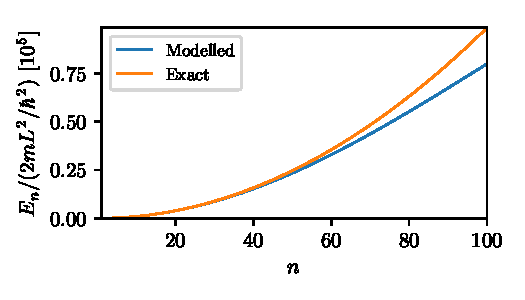
\includegraphics{figs/box_eigenvalues.pdf}%
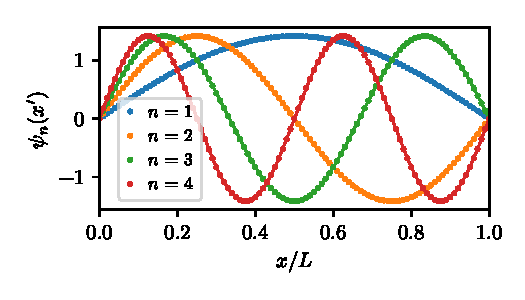
\includegraphics{figs/box_eigenvectors.pdf}%
\caption{Eigenvalues (left) and eigenfunctions (right) in an infinite well with $\Delta x' = 1/200$. \label{fig:box_solutions}}%
\end{figure}

In \cref{fig:box_time_psi0} the time development of the particle in a box is plotted for the initial condition $\Psi_0 = \psi_0$, the first eigenfunction.

\begin{figure}[ht!]%
\centering%
% 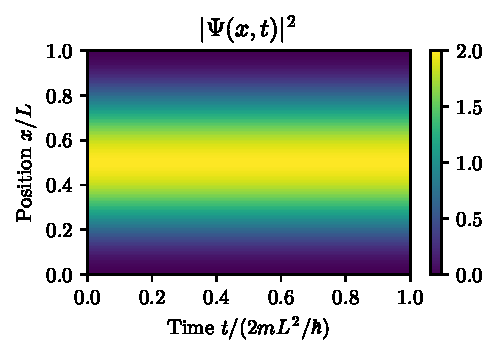
\includegraphics{figs/box_psi0_prob.pdf}\\%
% 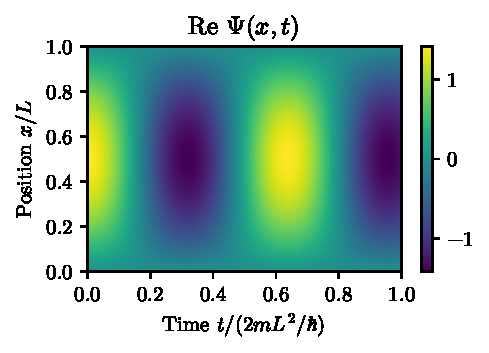
\includegraphics{figs/box_psi0_real.pdf}%
% 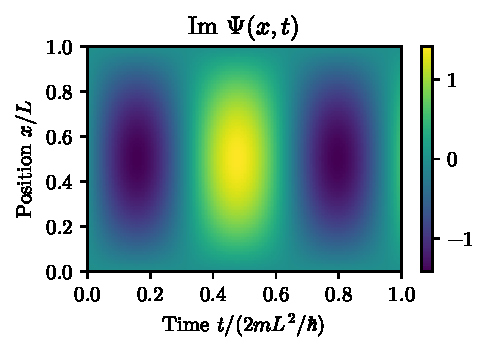
\includegraphics{figs/box_psi0_imag.pdf}%
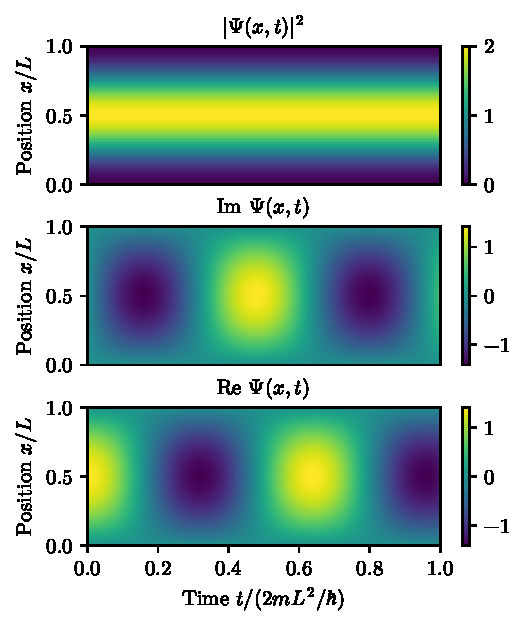
\includegraphics[width=0.99\textwidth]{figs/box_psi0.pdf}% single figure
\caption{Time-development of particle in a well with initial condition $\Psi_0(x',t'=0) = \psi_0$ and $\Delta x' = 1/200$ and $\Delta t' = 1/2000$. \label{fig:box_time_psi0}}%
\end{figure}

Using a delta function as initial condition $\Psi_0(x) = \delta(x - 1/2)$ fixes the initial position of the particle at $x=1/2$. This results in coefficients
\begin{equation}
    \alpha_n = \int \psi_n^{*}(x)\delta(x - 1/2) \dif x = \psi_n^{*}(x=1/2),
\end{equation}
which means that the initial wave function will be a combination of all eigenfunctions $\psi_n$'s. To properly represent this we need to include an infinite number of eigenfunctions. Further, since we have an exact position (with \emph{infinite certainty}) means that we have \emph{infinite uncertainty} in the momentum of the particle, following the uncertainty princinple. This means that any results for $t>0$ will not make any sense. Now, the numerical simulations doesn't know that this is not possible, so it willingly spits out results like the ones in \cref{fig:box_time_deltaf}. The simulations can not use an infinite number of eigenfunctions to represent the initial condition, so in practice we are probably seeing the results of using a bad approximation of a triangle wave or a Gaussian as initial condition.

\begin{figure}[ht!]%
\centering%
% 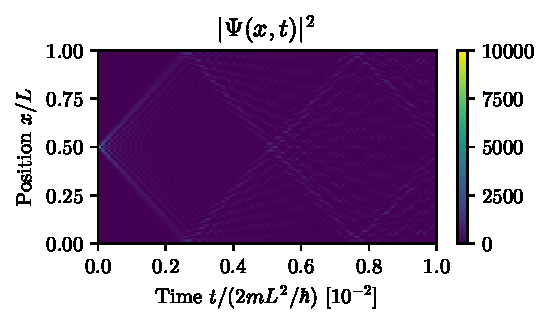
\includegraphics{figs/box_deltaf_prob.pdf}\\% % TOOD: Can remove this top figure if we need more space
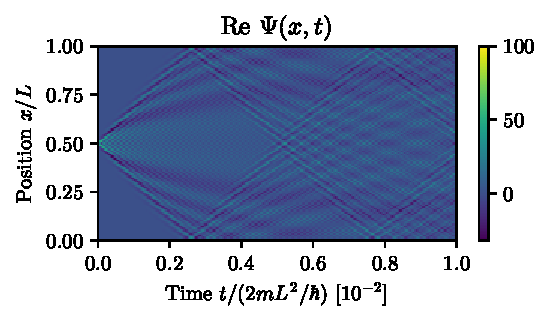
\includegraphics[width=0.49\textwidth]{figs/box_deltaf_real.pdf}%
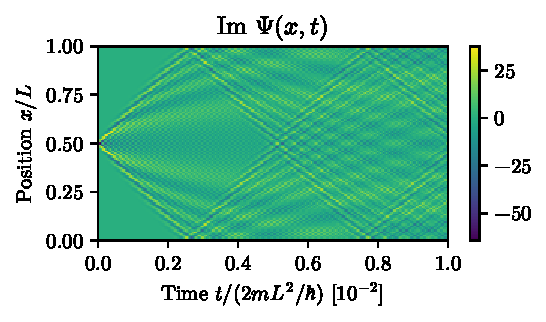
\includegraphics[width=0.49\textwidth]{figs/box_deltaf_imag.pdf}%
\caption{Time-development of particle in a well with initial condition $\Psi_0(x',t'=0) = \delta(x' - 1/2)$ and $\Delta x' = 1/200$ and $\Delta t' = 10^{-5}$. \label{fig:box_time_deltaf}}%
\end{figure}

\subsection*{Double well}
In \cref{fig:double_well_solutions} we have plots of the first three eigenfunctions of the double well (right), and the first eigenvalues. We see that the first excited state ($n=2$) has nearly the same wave function as the ground state, but with odd parity (the blue line for $n=1$ is hidden under the orange line for $n=2$ in the left half of the plot).
\begin{figure}[ht!]%
\centering%
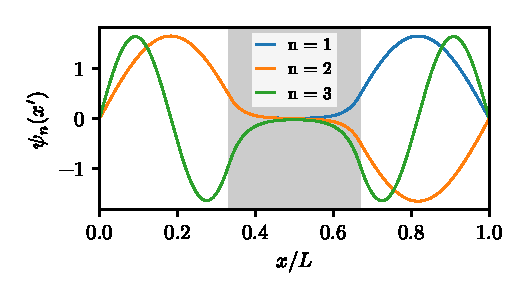
\includegraphics{figs/double_eigenfunctions.pdf}%
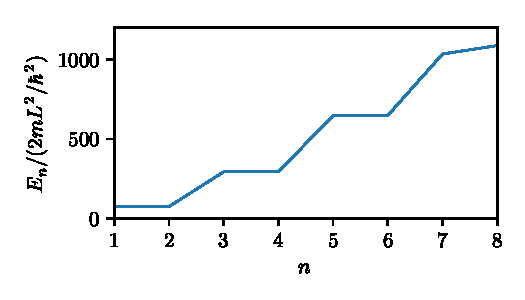
\includegraphics{figs/double_eigenvalues.pdf}%
\caption{Eigenfunctions (left) and eigenvalues (right) in a double well with $\Delta x' = 1/1000$ and $\nu_0 = 1000$. The middle barrier is indicated by the central gray area. \label{fig:well_solutions}}%
\end{figure}

The first 6 eigenvalues are given below. We see that the first excited state ($\lambda_2$) is \emph{nearly} degenerate with the ground state ($\lambda_1$), and similarly for $\lambda_3$ and $\lambda_4$, and $\lambda_5$ and $\lambda_6$. The states are not fully degenerate because we cannot have degeneracy in a 1D system like this.
\begin{center}
\begin{tabular}{ccc}
% \hline
$\lambda_1$ = 73.8663877 & $\lambda_2$ = 293.2169877 & $\lambda_4$ = 647.6674955 \\
$\lambda_2$ = 73.8683378 & $\lambda_3$ = 293.2410202 & $\lambda_5$ = 648.1536705
% \\\hline
\end{tabular}
\end{center}

In \cref{fig:double_well_solutions} plots of the probability density is given. We see that the probability density is concentrated the left side of the barrier at $t'=0$, and that it tunnels through the barrier and is fully concentrated on the right side of the barrier at $T = t' = \pi/(\lambda_2 - \lambda_1)$. The tunnelling time $T$ is the (half) period of the exponential of \cref{eq:time_evolution_expansion}.
\begin{figure}[ht!]%
\centering%
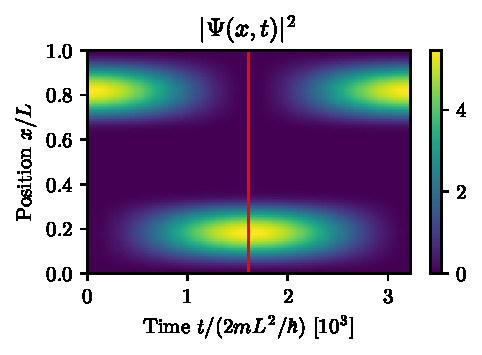
\includegraphics{figs/double_twopsi_prob.pdf}%
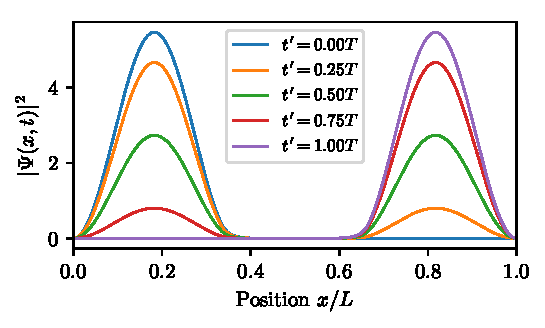
\includegraphics{figs/double_twopsi_prob_1d.pdf}%
\caption{Time evolution of the double well with initial condition $\Psi_0 = 1/\sqrt(2)(\psi_1 + \psi_2)$, $\Delta x' = 1/1000$ and $\nu_0 = 1000$. $T$ is the tunnelling time $t' = \pi/(\lambda_2 - \lambda_1)$, and is indicated by the red vertical line in the left figure. \label{fig:double_well_solutions}}%
\end{figure}

\subsubsection*{Root-finding}
It can be shown that the eigenvectors of the Hamiltonian with energies $0 < \lambda < \nu_0$ are given by the equation
\begin{equation}
    f(\lambda) = e^{\kappa/3}\sbr{\kappa\sin\del{\frac{k}{3}} + k\cos\del{\frac{k}{3}}}^2 - e^{-\kappa/3}\sbr{\kappa\sin\del{\frac{k}{3}} - k\cos\del{\frac{k}{3}}}^2 = 0,
    \label{eq:roots}
\end{equation}
where $k = \sqrt{\lambda}$ and $\kappa = \sqrt{\nu_0 - \lambda}$.

We find the roots of \cref{eq:roots} using the function \pyinline{scipy.optimize.root} from the \python-package \texttt{SciPy}, with the default \verb!hybr! method. This uses a modification of the Powell's hybrid method\cite{powell1970hybrid} implemented in MINPACK’s \verb!hybrd! and \verb!hybrj! routines. Other methods can be selected using the \verb!method! argument, but we found the default method to give sufficient results. We use the eigenvalues $\lambda_1$ to $\lambda_6$ from the previous section as starting points for the function. 

The resulting roots are listed below, and a plot of \cref{eq:roots} with the roots indicated by vertical lines is shown in \cref{fig:roots}. We see that the roots of \cref{eq:roots} doesn't perfectly agree with the eigenvalues found before.

\begin{center}
\begin{tabular}{ccc}
% \hline
$\lambda_1$ = 73.9375329 &$\lambda_3$ = 293.5161981 &$\lambda_5$ = 648.7502782 \\
$\lambda_2$ = 73.9356002 &$\lambda_4$ = 293.4923150 &$\lambda_6$ = 648.2643732
% \\\hline
\end{tabular}
\end{center}

\begin{figure}[ht!]%
\centering%
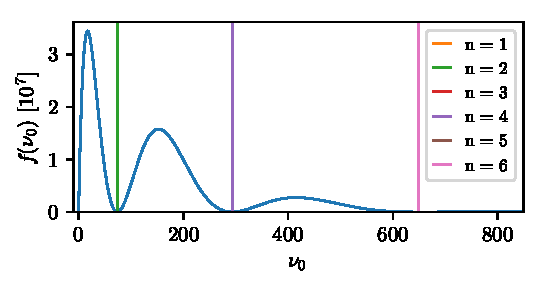
\includegraphics{figs/roots_with_roots.pdf}%
% 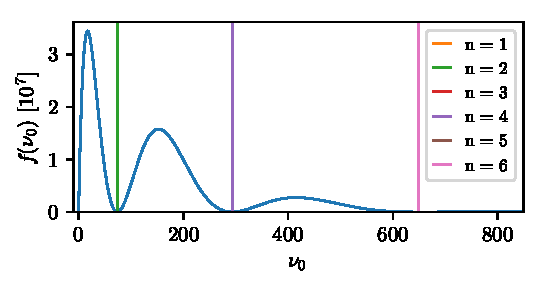
\includegraphics{figs/roots_with_roots.pdf}%
\caption{Plot of \cref{eq:roots}, with the roots indicated by vertical lines. The lines for $n=1$ and $n=2$ overlap, as does $n=3$ and $n=4$ etc. \label{fig:roots}}%
\end{figure}

In \cref{fig:eigenvalues_roots} we have plots of the number of eigenstates with eigenvalues lower than the barrier height $\nu_0$. We find that the barrier height that separates having none and one such eigenstate is approximately $\nu_0 = 22.2$.
\begin{figure}[ht!]%
\centering%
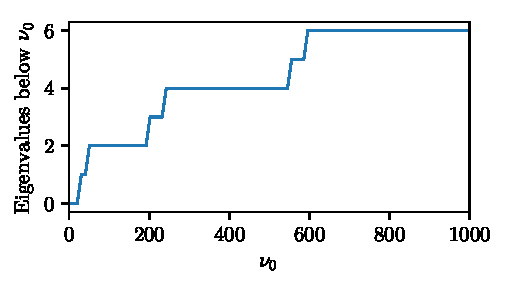
\includegraphics{figs/roots_all.pdf}%
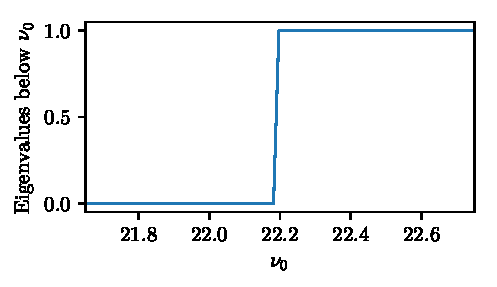
\includegraphics{figs/roots_details.pdf}%
\caption{Plots of the number of eigenstates with eigenvalues less than the barrier height $\nu_0$, as function of $\nu_0$. \label{fig:eigenvalues_roots}}%
\end{figure}

\subsection*{Finite difference time evolution}
\begin{itemize}
    % \item \sout{Plot eigenvalues $\lambda_n$ as function of $n$, discuss results}
    % \item \sout{Plot time evolution with tunnelling, discuss tunnelling and why it happens at time $\pi/(\lambda_2 - \lambda_1)$}
    % \item \sout{(Plot $f(\lambda)$ from eq. 3.4?)}
    % \item \sout{Find roots/eigenvalues from eq. 3.4}
    % \item \sout{compare roots to eigenvalues from solving TISE}
    % \item \sout{Estimate barrier height that separates having one eigenstate with $\lambda_n < \nu_0$ and having no such states}
    \item (Plot time evolution using Euler scheme for TISE (eq. 3.6))
    \item Plot time evolution using C-N scheme for TISE (eq. 3.8)
    \item Time-dependent Hamiltonian!! \hl{Discuss when it's advantageous to use step-by-step time evolution. Does it depend on the initial condition? Make a few hypotheses, and test the ideas.}
\end{itemize}

\subsection*{Two-level double well system}

In the left plot in \cref{fig:detuning1} there is a plot of the two lowest eigenvalues $\lambda_1$ and $\lambda_2$ as function of the potential $\nu_r$. In the right plot the two lowest eigenfunctions are plotted for positive and negative $\nu_r$. We see that the ground state $\psi_1$ is localized at the left side for positive $\nu_r$, and mostly located at the right side for negative $\nu_r$, and vice versa for the excited state $\psi_2$.
\begin{figure}[ht!]%
\centering%
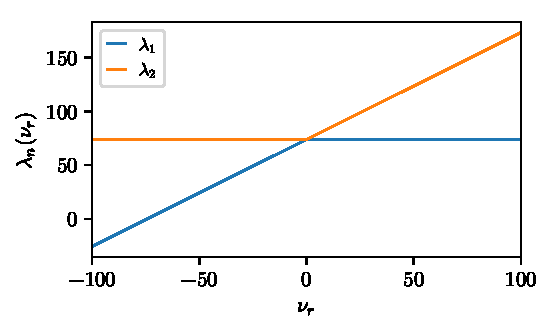
\includegraphics{figs/detuning_4_1.pdf}%
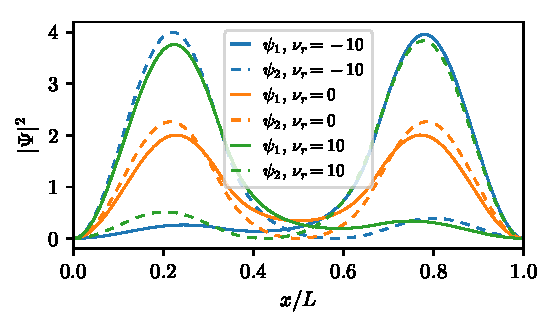
\includegraphics{figs/detuning_localization.pdf}%
\caption{(left) Plot of the two lowest eigenvalues as function of $\nu_r$ with $\Delta x' = 1/1000$, and (right) localization of ground state with positive and negative $\nu_r$. \label{fig:detuning1}}%
\end{figure}

\section*{Conclusion}

\printbibliography[title=References]

\end{document}